\documentclass[11pt]{article}
\usepackage[margin=1in]{geometry}
\usepackage[T1]{fontenc}
\usepackage{lmodern,microtype,booktabs,graphicx,xcolor,hyperref,amsmath,siunitx,tabularx,enumitem}
\usepackage[numbers,sort&compress]{natbib}
\hypersetup{colorlinks=true,linkcolor=blue!50!black,citecolor=blue!50!black,urlcolor=blue!50!black}

% --- drafting helpers -------------------------------------------------------
\newcommand{\todo}[1]{\textcolor{red!70!black}{\textbf{[TODO:} #1\textbf{]}}}
\newcommand{\note}[1]{\textcolor{blue!60!black}{\textit{[#1]}}}
\newcommand{\go}[2]{\textsf{#2} (\texttt{#1})}          % \go{GO:0005515}{protein binding}
\newcommand{\gene}[1]{\textit{#1}}
\newcommand{\act}[1]{\textsc{\MakeLowercase{#1}}}        % \act{REMOVE}
\newcommand{\proj}[1]{\texttt{projects/#1}}              % repo provenance for a deep-dive number

% All corpus numbers come from here (scripts/compute_stats.py). Never type them by hand.
% generated by scripts/compute_stats.py -- do not edit
\newcommand{\accAuthorCuratorStatement}{71.7}
\newcommand{\accCACAO}{52.3}
\newcommand{\accComplexPortal}{68.8}
\newcommand{\accEXP}{77.8}
\newcommand{\accElectronicIea}{48.0}
\newcommand{\accExperimental}{59.8}
\newcommand{\accHDA}{42.4}
\newcommand{\accHighThroughput}{43.4}
\newcommand{\accIBA}{70.1}
\newcommand{\accIDA}{67.5}
\newcommand{\accIEA}{48.0}
\newcommand{\accIEP}{13.6}
\newcommand{\accIGI}{45.8}
\newcommand{\accIMP}{46.3}
\newcommand{\accIPI}{57.4}
\newcommand{\accISO}{33.0}
\newcommand{\accISS}{42.4}
\newcommand{\accNAS}{57.7}
\newcommand{\accNoDataNd}{73.2}
\newcommand{\accPhylogeneticIba}{70.1}
\newcommand{\accPseudoCAP}{57.1}
\newcommand{\accRCA}{73.7}
\newcommand{\accSequenceOrthology}{43.9}
\newcommand{\accSynGO}{32.6}
\newcommand{\accSynGOUCL}{25.0}
\newcommand{\accTAS}{74.3}
\newcommand{\aspectMatched}{99.5}
\newcommand{\modEXP}{7.9}
\newcommand{\modHDA}{3.0}
\newcommand{\modIBA}{7.1}
\newcommand{\modIDA}{6.9}
\newcommand{\modIEA}{14.1}
\newcommand{\modIEP}{2.5}
\newcommand{\modIGI}{5.8}
\newcommand{\modIMP}{6.5}
\newcommand{\modIPI}{8.0}
\newcommand{\modISO}{8.7}
\newcommand{\modISS}{6.5}
\newcommand{\modNAS}{9.4}
\newcommand{\modRCA}{7.0}
\newcommand{\modTAS}{5.3}
\newcommand{\nAnn}{329,130}
\newcommand{\nAnnNoPB}{275,580}
\newcommand{\nAuthorCuratorStatement}{42,528}
\newcommand{\nCACAO}{709}
\newcommand{\nComplexPortal}{6,930}
\newcommand{\nCoreFns}{15,718}
\newcommand{\nEXP}{6,369}
\newcommand{\nElectronicIea}{75,108}
\newcommand{\nExperimental}{93,746}
\newcommand{\nHDA}{5,248}
\newcommand{\nHighThroughput}{5,843}
\newcommand{\nIBA}{28,575}
\newcommand{\nIDA}{49,444}
\newcommand{\nIEA}{75,108}
\newcommand{\nIEP}{1,680}
\newcommand{\nIGI}{4,583}
\newcommand{\nIMP}{25,246}
\newcommand{\nIPI}{6,424}
\newcommand{\nISO}{11,250}
\newcommand{\nISS}{13,246}
\newcommand{\nKnowledgeGaps}{1,347}
\newcommand{\nNAS}{6,330}
\newcommand{\nNew}{5,716}
\newcommand{\nNoDataNd}{425}
\newcommand{\nOrgFolders}{345}
\newcommand{\nPB}{53,550}
\newcommand{\nPhylogeneticIba}{28,595}
\newcommand{\nProposedTerms}{795}
\newcommand{\nPseudoCAP}{324}
\newcommand{\nRCA}{4,093}
\newcommand{\nRefs}{193,275}
\newcommand{\nReviews}{10,505}
\newcommand{\nSequenceOrthology}{29,335}
\newcommand{\nSynGO}{530}
\newcommand{\nSynGOUCL}{8}
\newcommand{\nTAS}{35,467}
\newcommand{\pbModify}{21.3}
\newcommand{\pbRemove}{50.1}
\newcommand{\pctAccept}{48.2}
\newcommand{\pctAcceptNoPB}{57.5}
\newcommand{\pctChangedAll}{27.0}
\newcommand{\pctChangedNoPB}{16.1}
\newcommand{\pctKeepAsNonCore}{22.7}
\newcommand{\pctKeepAsNonCoreNoPB}{24.5}
\newcommand{\pctMarkAsOverAnnotated}{6.0}
\newcommand{\pctMarkAsOverAnnotatedNoPB}{4.9}
\newcommand{\pctModify}{10.8}
\newcommand{\pctModifyNoPB}{8.7}
\newcommand{\pctPB}{16.3}
\newcommand{\pctRejectedAll}{15.6}
\newcommand{\pctRejectedNoPB}{6.6}
\newcommand{\pctRemove}{9.6}
\newcommand{\pctRemoveNoPB}{1.7}
\newcommand{\pctTooGeneral}{0.6}
\newcommand{\pctTooGeneralNoPB}{0.8}
\newcommand{\pctUndecided}{2.1}
\newcommand{\pctUndecidedNoPB}{1.9}
\newcommand{\rejAuthorCuratorStatement}{4.2}
\newcommand{\rejCACAO}{6.8}
\newcommand{\rejComplexPortal}{5.3}
\newcommand{\rejEXP}{1.2}
\newcommand{\rejElectronicIea}{9.7}
\newcommand{\rejExperimental}{4.1}
\newcommand{\rejHDA}{15.2}
\newcommand{\rejHighThroughput}{14.9}
\newcommand{\rejIBA}{5.8}
\newcommand{\rejIDA}{3.2}
\newcommand{\rejIEA}{9.7}
\newcommand{\rejIEP}{31.1}
\newcommand{\rejIGI}{3.8}
\newcommand{\rejIMP}{4.9}
\newcommand{\rejIPI}{3.9}
\newcommand{\rejISO}{12.0}
\newcommand{\rejISS}{7.1}
\newcommand{\rejNAS}{9.1}
\newcommand{\rejNoDataNd}{10.1}
\newcommand{\rejPhylogeneticIba}{5.8}
\newcommand{\rejPseudoCAP}{13.9}
\newcommand{\rejRCA}{10.8}
\newcommand{\rejSequenceOrthology}{9.6}
\newcommand{\rejSynGO}{1.5}
\newcommand{\rejSynGOUCL}{0.0}
\newcommand{\rejTAS}{3.3}


\title{Agentic review uncovers large systematic errors in biological knowledge bases}
\author{\todo{authors} \\ \small AI Gene Review consortium \todo{affiliations}}
\date{\todo{date}}

\begin{document}
\maketitle

\begin{abstract}
Biological knowledge bases such as the Gene Ontology (GO) annotation corpus underpin enrichment
analysis, function prediction and the training of machine-learning models, yet their
correctness is rarely audited after an annotation is made. We built an agentic review system
in which a large-language-model agent, constrained by a typed schema, a cached literature
corpus and verbatim-quote validation, re-adjudicates every existing GO annotation for a gene
against the primary literature, sequence analysis and curation guidelines, and records a
structured action (\act{ACCEPT}, \act{KEEP\_AS\_NON\_CORE}, \act{MODIFY}, \act{REMOVE},
\act{MARK\_AS\_OVER\_ANNOTATED}, \ldots) with its justification. Across \nReviews{} gene reviews
in \nOrgFolders{} taxa we adjudicated \nAnn{} annotations, citing \nRefs{} references.
\pctChangedAll\% of annotations were changed or rejected (\pctChangedNoPB\% after excluding the
uninformative \emph{protein binding} term). Errors are not uniformly distributed: they
concentrate in specific pipelines (\todo{top pipelines}), specific evidence types (expression
patterns, orthology transfer), and specific ontology regions. We describe ten systematic error
classes in depth---from keyword mappings that conflate regulation with participation to
pseudoenzymes that inherit catalytic activity---several of which have already led to term
obsoletions and pipeline retirements upstream. \todo{one sentence on validation against expert
curators.} Agentic review is a practical route to continuous, auditable quality control of
community knowledge bases.
\end{abstract}

\section{Introduction}\label{sec:intro}

\note{Arc: (1) knowledge bases are infrastructure; (2) they are written once and rarely re-read;
(3) errors are systematic because most content is produced by pipelines, and errors propagate
(IBA, orthology, ML training sets); (4) previous audits were small or statistical (RAR, CAFA,
Schnoes 2009); (5) LLM agents can now read papers and reason about ontologies, but naive LLM
curation hallucinates; (6) we show a constrained agentic system that scales, is auditable, and
finds errors that matter.}

\paragraph{Knowledge bases as infrastructure.} GO \citep{todo-go2023} \todo{scale: terms,
annotations, fraction IEA in UniProt-GOA}. Used for enrichment, CAFA benchmarks, and as labels for
protein language models \todo{cite}.

\paragraph{Write once, read rarely.} An annotation is a claim tied to a paper or pipeline at a
date. Ontology changes, retractions, and new evidence do not trigger re-review. Prior work on
misannotation: Schnoes et al.\ 2009 (enzyme superfamilies) \todo{cite}; taxon-specific rate
ratios (RAR; \citealp{todo-wei2020}); GO's own quality-control rules \todo{cite}.

\paragraph{Why errors are systematic.} Most annotations are produced by a small number of
mappings (InterPro2GO, UniProt keywords, ARBA, Ensembl Compara, PAINT/IBA). A single bad mapping
or node placement is copied to every protein that matches it. Errors are therefore correlated, and
correlated errors are invisible to evaluations that treat existing annotations as ground truth.

\paragraph{What is new here.} \todo{contributions list:}
\begin{enumerate}[nosep]
  \item A constrained agentic review architecture (schema, cached sources, verbatim quotes,
        policy validators, append-only provenance) that makes LLM curation auditable.
  \item A corpus of \nReviews{} reviews and \nAnn{} adjudicated annotations, released openly.
  \item Corpus-wide error rates stratified by evidence type, pipeline, aspect and taxon.
  \item Twelve deep dives into systematic error classes, with upstream fixes.
\end{enumerate}

\section{How annotations are made: experiment, inference and propagation}\label{sec:landscape}

\note{Explainer section for a general reader. One figure: the provenance graph of a single
annotation (paper $\rightarrow$ curator $\rightarrow$ GAF row; or InterPro entry $\rightarrow$
InterPro2GO $\rightarrow$ every matching protein; or PAINT IBD at an ancestral node $\rightarrow$
IBA on all descendants). Use one gene as the running example \todo{pick: e.g.\ a kinase with
EXP, IBA and IEA rows on the same term}.}

\subsection{Experimental annotations}
Curator reads a paper and asserts a term with an evidence code (IDA, IMP, IPI, IGI, IEP, EXP),
plus high-throughput variants (HDA, HMP, \ldots). Strength: grounded in data. Weakness: the
\emph{inference} from assay to function (an interaction is not an activity; a knockout phenotype is
necessity, not participation; expression is not function).

\subsection{Phylogenetic annotations (IBA)}
PAINT curators place IBD assertions at nodes of PANTHER family trees after inspecting all
experimental annotations of descendants; IBA rows follow mechanically \citep{todo-gaudet2011}.
An IBA is a considered evolutionary judgement, not a similarity transfer. Failure modes: node
placed too deep; neo-functionalised subfamily; pseudoenzymes; cross-kingdom extension.

\subsection{Electronic annotations (IEA)}
Mappings from signatures to terms: InterPro2GO, UniProt keywords (KW2GO), subcellular location,
EC2GO, Rhea2GO, UniRule, ARBA association rules, Ensembl Compara orthology, TreeGrafter, GO's own
logical inference. Unreviewed, applied at proteome scale, refreshed with each release.

\subsection{Author statements and other codes}
TAS/NAS (including Reactome), IC, ISS/ISO/ISA, RCA, ND.

\begin{table}[t]\centering\small
\caption{Composition of the reviewed corpus by evidence class \todo{add share of all UniProt-GOA
for comparison, to show how representative the sample is}.}
\label{tab:composition}
\todo{generate from compute\_stats.py: n rows per class and per aspect, \% of corpus.}
\end{table}
     % 2. How GO annotations are made: EXP vs IEA vs IBA
\section{An agentic review system}\label{sec:system}

\begin{figure}[t]\centering
\resizebox{\linewidth}{!}{% Fig: the agentic review system. Included from sections/system.tex.
\begin{tikzpicture}[
  font=\sffamily\scriptsize, node distance=4mm and 3.2mm,
  box/.style={draw=black!45, rounded corners=2pt, fill=#1, align=center, inner sep=3pt, minimum height=11mm, text width=19mm},
  box/.default=white,
  src/.style={box=blue!6}, agent/.style={box=green!8}, check/.style={box=orange!10}, upbox/.style={box=red!6},
  arr/.style={-{Stealth[length=2mm]}, draw=black!55, thick}]
\node[src] (fetch) {\textbf{Fetch}\\UniProt record, GOA rows, cached papers};
\node[src, right=of fetch] (dr) {\textbf{Deep research}\\several providers, cited reports};
\node[agent, right=of dr] (rev) {\textbf{Agent review}\\action + reason + verbatim quotes per row};
\node[check, right=of rev] (val) {\textbf{Validate}\\schema, term ids, quotes, policies};
\node[check, right=of val] (pr) {\textbf{Pull request}\\review, merge, history record};
\node[upbox, below=6mm of val, text width=40mm, minimum height=9mm] (up) {\textbf{Upstream}: source defects, NOT candidates,\\proposed terms, mapping and rule edits};
\node[agent, below=6mm of dr, text width=40mm, minimum height=9mm] (tools) {\textbf{Tools}: OLS, PubMed, UniProt, PANTHER/PAINT,\\InterPro, reproducible bioinformatics};
\draw[arr] (fetch) -- (dr); \draw[arr] (dr) -- (rev); \draw[arr] (rev) -- (val); \draw[arr] (val) -- (pr);
\draw[arr] (val.north) to[bend right=25] node[above, font=\sffamily\tiny]{fails: revise} (rev.north);
\draw[arr] (pr.south) |- (up.east);
\draw[arr] (tools.east) -| (rev.south);
\end{tikzpicture}
}
\caption{The agentic review system. Each gene review passes fetch, deep research, agent review,
validation and pull-request review; validated findings feed reports to upstream resources.}
\label{fig:system}
\end{figure}

\subsection{The review document}
One YAML document per gene (LinkML schema, \texttt{gene\_review.yaml}): a standalone
description, the references used, one entry per existing annotation with an action, summary,
reason and \texttt{supported\_by} quotes, the gene's \emph{core functions} (MF + process +
location + complex), proposed new terms, knowledge gaps, suggested experiments.

\subsection{The action vocabulary}
\begin{description}[nosep,font=\normalfont\scshape]
  \item[accept] correct and part of the core function.
  \item[keep\_as\_non\_core] correct and as precise as warranted, but peripheral.
  \item[modify] sound but a better term exists (more specific, or sign/lateral correction);
        carries proposed replacements.
  \item[too\_general] true but entailed by a more specific term in the review.
  \item[mark\_as\_over\_annotated] not strictly false, but an over-reach.
  \item[remove] unlikely to be correct on the combined evidence.
  \item[undecided] evidence insufficient or inaccessible.
  \item[new] proposed annotation absent from GOA.
\end{description}
\note{Make explicit: actions judge \emph{claims}, not evidence codes; rows sharing a term must be
consistent; ``correct but general'' is \act{MODIFY} not \act{KEEP\_AS\_NON\_CORE}.}

\subsection{Guardrails against hallucination}
\begin{itemize}[nosep]
  \item Cached sources only; every \texttt{supporting\_text} must be a verbatim substring of the
        cached paper, UniProt record, Reactome entry or analysis file.
  \item Reference titles are checked against the fetched record (catches transposed PMIDs).
  \item Author-supplied term ids are validated against ontology branches; GOA ids are trusted.
  \item Policy validators encode curation conventions (protein binding, ND, root organelle
        terms, IBA reading, ``do not add what curators declined to add'').
  \item Experimental annotations whose full text is not cached are not removed (\act{UNDECIDED}).
  \item Bioinformatics analyses are reproducible scripts; results never hardcoded.
  \item Every change is a reviewed pull request with an append-only history record.
\end{itemize}

\subsection{Gene selection}
\todo{Describe honestly: not a random sample. Mix of (a) whole-proteome campaigns (e.g.\
\textit{P. putida}, \textit{S. pombe}, yeast), (b) thematic projects (proteostasis, immunity,
\ldots), (c) term-centric audits (all annotations to a term slated for obsoletion), (d) human
gene sets. Quantify selection; report results per campaign type to show robustness.}

\subsection{Models and agents}
\todo{Which agent frameworks and model versions, over what period; deep-research providers;
cost per gene; wall-clock.}
        % 3. The agentic review system and its action vocabulary
\section{Corpus-wide results}\label{sec:overview}

\subsection{Scale}
\nReviews{} reviews in \nOrgFolders{} taxon folders; \nAnn{} adjudicated existing annotations
(aspect resolved for \aspectMatched\% of rows); \nNew{} proposed new annotations; \nCoreFns{} core
functions; \nRefs{} reference entries; \nProposedTerms{} proposed GO terms; \nKnowledgeGaps{}
knowledge gaps. \todo{distribution of annotations per gene; taxon breakdown figure.}

\subsection{Overall action distribution}
\pctAccept\% \act{ACCEPT}, \pctKeepAsNonCore\% \act{KEEP\_AS\_NON\_CORE}, \pctModify\% \act{MODIFY},
\pctTooGeneral\% \act{TOO\_GENERAL}, \pctMarkAsOverAnnotated\% \act{MARK\_AS\_OVER\_ANNOTATED},
\pctRemove\% \act{REMOVE}, \pctUndecided\% \act{UNDECIDED}.
\emph{Protein binding} (\go{GO:0005515}{protein binding}) alone is \nPB{} rows (\pctPB\% of the
corpus) and is handled by policy (\S\ref{sec:dd-pb}); excluding it, \pctRejectedNoPB\% of
annotations are rejected (\act{REMOVE} or \act{MARK\_AS\_OVER\_ANNOTATED}) and \pctChangedNoPB\%
are changed in any way.

\note{Framing: a per-row error rate in the single digits is not the story. The story is that the
errors are \emph{concentrated} and \emph{systematic}: specific pipelines, codes and ontology
regions carry rejection rates several-fold above baseline, and because each is a mapping applied
proteome-wide, the absolute number of affected annotations in UniProt-GOA is large.
\todo{extrapolate: rejection rate per pipeline $\times$ pipeline size in current GOA.}}

\subsection{Errors by evidence class}
\begin{figure}[t]\centering
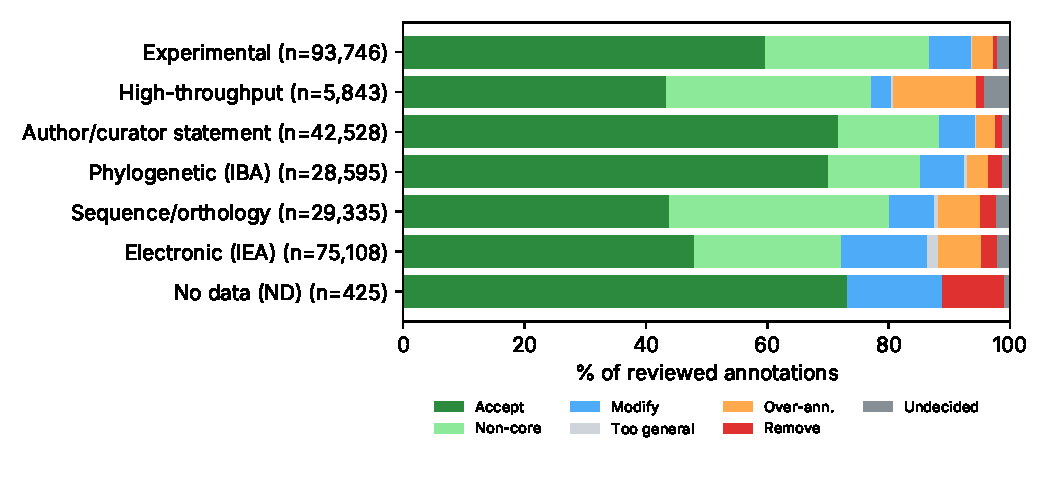
\includegraphics[width=\linewidth]{figures/action_by_evidence.pdf}
\caption{Review actions by evidence class (excluding protein binding).}
\label{fig:evidence}
\end{figure}

\begin{table}[t]\centering\scriptsize\setlength{\tabcolsep}{3pt}
\caption{Review actions (\% of rows) by evidence class, excluding protein binding.}
\label{tab:egroup}
% generated by scripts/compute_stats.py -- do not edit
\begin{tabular}{lrrrrrrrr}\toprule
Evidence class & $n$ & Accept & Non-core & Modify & Too general & Over-ann. & Remove & Undecided \\ \midrule
Experimental & 93,746 & 59.8 & 27.0 & 6.8 & 0.3 & 3.4 & 0.7 & 2.0 \\
High-throughput & 5,843 & 43.4 & 33.8 & 3.2 & 0.3 & 13.6 & 1.3 & 4.2 \\
Author/curator statement & 42,528 & 71.7 & 16.6 & 5.9 & 0.2 & 3.1 & 1.1 & 1.3 \\
Phylogenetic (IBA) & 28,595 & 70.1 & 15.1 & 7.1 & 0.6 & 3.5 & 2.3 & 1.2 \\
Sequence/orthology & 29,335 & 43.9 & 36.2 & 7.5 & 0.7 & 7.0 & 2.6 & 2.2 \\
Electronic (IEA) & 75,108 & 48.0 & 24.3 & 14.1 & 1.8 & 7.0 & 2.7 & 2.1 \\
No data (ND) & 425 & 73.2 & 0.0 & 15.8 & 0.0 & 0.0 & 10.1 & 0.9 \\
\bottomrule
\end{tabular}

\end{table}

Observations to develop:
\begin{itemize}[nosep]
  \item IBA is accepted at \accIBA\% (rejected \rejIBA\%), on a par with direct assays (IDA
        \accIDA\%) and well above other homology transfer (ISO \accISO\%, rejected \rejISO\%;
        ISS \accISS\%). Phylogenetically curated propagation behaves like experimental evidence;
        pairwise orthology transfer does not.
  \item Expression-pattern evidence (IEP) is the weakest experimental code (accepted \accIEP\%,
        rejected \rejIEP\%): expression is read as participation.
  \item High-throughput direct assays (HDA) are rejected at \rejHDA\% \todo{check: localisation proteomics?}.
  \item IEA is modified at \modIEA\% (vs IDA \modIDA\%): electronic terms are often right in
        kind but wrong in grain.
  \item Mutant phenotypes (IMP, IGI) are accepted at only \accIMP\% / \accIGI\%, with most of the
        remainder non-core: necessity is not participation.
\end{itemize}

\subsection{Errors by IEA pipeline}
\begin{table}[t]\centering\scriptsize\setlength{\tabcolsep}{3pt}
\caption{Review actions by electronic pipeline (GO\_REF), excluding protein binding.}
\label{tab:iea}
% generated by scripts/compute_stats.py -- do not edit
\begin{tabular}{lrrrrrrrr}\toprule
IEA pipeline & $n$ & Accept & Non-core & Modify & Too general & Over-ann. & Remove & Undecided \\ \midrule
Ensembl Compara orthology & 17,048 & 27.7 & 46.0 & 5.7 & 0.5 & 12.0 & 2.6 & 5.6 \\
InterPro2GO & 15,679 & 41.1 & 13.3 & 30.0 & 4.0 & 7.2 & 3.6 & 0.8 \\
Combined automated (UniProt) & 15,152 & 74.2 & 11.6 & 9.4 & 0.9 & 2.4 & 0.8 & 0.6 \\
UniProt subcellular location2GO & 9,349 & 63.0 & 25.5 & 7.1 & 0.6 & 2.1 & 0.6 & 1.1 \\
ARBA & 8,736 & 39.0 & 28.9 & 15.8 & 3.3 & 9.2 & 2.1 & 1.6 \\
UniProt keyword2GO & 2,906 & 44.4 & 14.6 & 22.1 & 2.7 & 9.3 & 6.6 & 0.3 \\
TreeGrafter & 1,501 & 43.7 & 22.9 & 9.6 & 0.9 & 8.6 & 10.4 & 4.0 \\
UniRule & 1,366 & 36.6 & 20.2 & 27.0 & 3.1 & 8.2 & 4.1 & 0.8 \\
GO logical inference & 1,154 & 35.8 & 23.7 & 10.0 & 0.3 & 14.0 & 14.0 & 2.3 \\
Rhea2GO & 832 & 60.9 & 19.7 & 10.7 & 0.8 & 4.9 & 1.3 & 1.6 \\
UniPathway2GO & 803 & 70.5 & 14.7 & 7.5 & 2.4 & 3.2 & 1.5 & 0.2 \\
EC2GO & 560 & 72.1 & 5.4 & 10.2 & 0.0 & 3.4 & 5.5 & 3.4 \\
\bottomrule
\end{tabular}

\end{table}
\note{Points: InterPro2GO is the most \act{MODIFY}-heavy (domain implies kind, not specificity);
GO logical inference and TreeGrafter have the highest rejection rates; Ensembl Compara orthology
has the lowest acceptance (most rows non-core or over-annotated, mainly BP from model-organism
phenotypes); UniProt-curated combined/subcellular-location rows are among the most reliable.}

\subsection{Errors by aspect and taxon}
\begin{table}[t]\centering\scriptsize\setlength{\tabcolsep}{3pt}
\caption{Review actions by GO aspect, excluding protein binding.}
\label{tab:aspect}
% generated by scripts/compute_stats.py -- do not edit
\begin{tabular}{lrrrrrrrr}\toprule
Aspect & $n$ & Accept & Non-core & Modify & Too general & Over-ann. & Remove & Undecided \\ \midrule
MF & 65,931 & 63.1 & 13.7 & 14.2 & 1.2 & 4.0 & 2.3 & 1.5 \\
BP & 106,286 & 42.8 & 36.1 & 8.1 & 0.9 & 7.6 & 1.8 & 2.6 \\
CC & 102,403 & 69.2 & 19.4 & 5.6 & 0.4 & 2.7 & 1.2 & 1.5 \\
\bottomrule
\end{tabular}

\end{table}
\todo{Biological process is the weak aspect (lowest acceptance); explain. Taxon table in
supplement (Table~\ref{tab:organism}).}

\subsection{Beyond existing annotations}
\todo{NEW annotations (\nNew): by aspect/evidence; proposed terms (\nProposedTerms); knowledge gaps
(\nKnowledgeGaps); source defects reported upstream; NOT candidates.}

\subsection{How reliable are the agent's calls?}
\todo{Essential for this title. Options: (a) blinded expert adjudication of a stratified random
sample of $\sim$500 decisions (per action $\times$ evidence class), reporting precision of
\act{REMOVE}/\act{MARK\_AS\_OVER\_ANNOTATED}; (b) agreement with upstream: fraction of
reported removals since acted on by GO/UniProt/MODs (cf.\ RAR re-examination); (c) re-review
stability across models/runs; (d) PR-review correction rate from history records.}
      % 4. Corpus-wide results
\section{Deep dives: twelve systematic error classes}\label{sec:deepdives}
\note{Each deep dive follows the same template: (i) the error class in one sentence;
(ii) why the pipeline produces it; (iii) scale in our corpus, from a reproducible query;
(iv) one or two worked genes; (v) what changed upstream (term obsoleted, mapping repointed,
pipeline retired, NOT filed) or what should. Numbers marked \proj{} are taken from the
project page and must be re-derived by a script under \texttt{paper/scripts/} before
submission.}

\note{Candidate list (pick ten; alternates at the end): protein binding; keyword mappings;
IBA; domain mappings (InterPro2GO/ARBA); pseudoenzymes and NOTs; enzyme specificity; sign
errors; ontology-driven errors (chaperones, precomposed terms, obsoletions); citations;
wrong entities (gene models, isoforms, microproteins). Alternates: ND and the dark proteome;
cellular-component granularity (organelles); ML predictors trained on the errors
(ProtNLM, BioReason, GO-GPT); conserved-function recovery (FliI/SctN as ATP synthase);
whole-proteome bacterial review (\textit{P. putida}).}

\subsection{Experimental is not the same as functional: the distance from readout to activity}\label{sec:dd-assay}
\textbf{Claim.} Evidence codes say an experiment was done, not how close its readout sits to the
gene product's own activity. Expression changes (IEP), distal phenotypes and fractionation proteomics
are filed alongside reconstituted enzyme assays, and they are the main source of over-annotation
among experimental rows.
\textbf{Corpus.} IEP is the weakest experimental code (\accIEP\% accepted, \rejIEP\% rejected);
high-throughput direct assays (HDA) are rejected at \rejHDA\%; mutant phenotypes (IMP, IGI) are
accepted at only \accIMP\% / \accIGI\%, most of the rest kept as non-core.
\textbf{Projects.} \proj{ASSAY\_TO\_FUNCTION.md}: catalogue of 60 readout classes mined from cached
papers; molecular readouts license an MF term 77\% of the time (567/738) and phenotypic hub
readouts 8\% (90/1,087). \proj{BEHAVIOR.md}: 86\% of adjudicated behaviour annotations (169/197)
downgraded; accepted ones are sensory channels and receptors acting in the circuit.
\proj{IEP.md}: survey of all 25,401 IEP rows in UniProt-GOA. \proj{OMICS\_EVIDENCE.md}: locations
read from organelle proteomes hold up (63--89\% accepted) but vesicle and body-fluid proteomes do not
(6\%), and functions read from location or co-purification are unreliable under any code.
\textbf{Principle.} Necessity is not participation (the AGT/angiotensin-maturation comparator check).
\textbf{Message.} Downstream users who trust ``experimental'' and distrust ``electronic'' are
filtering on the wrong axis.

\subsection{Phylogeny mostly gets it right, but bad seeds spread}\label{sec:dd-iba}
\textbf{Claim.} IBA is the best-performing inferred evidence (\accIBA\% accepted, \rejIBA\% rejected),
because PAINT curators place functions at tree nodes after reading every descendant's evidence.
Its failures are structured: node placed too deep, neo-functionalised subfamilies, pseudoenzymes,
and above all a wrong \emph{seed}: one experimental annotation on one protein becomes an IBA on
every descendant.
\textbf{Projects.} \proj{IBA\_REVIEW.md}: 16 failure patterns, 79 worked cases; IBA too conservative
for core MF in human as well. \proj{PANTHER\_IBA\_REVIEW.md}: all 160 IBAs on 41 \textit{S.\ pombe}
genes rebuilt from source node; 148 kept. \proj{PSEUDOCAP.md}: of 109 \textit{P.\ aeruginosa} proteins
that are the \emph{sole} seed of a PAINT node term, 21 carry a wrong or indirect seed (catalase activity
on a heme exporter, a mistyped GO id on pilU, signal transduction on a signal synthase).
\proj{CACAO.md}: student community annotations (\nCACAO{} rows here, \accCACAO\% accepted).
\proj{TRANSCRIPTION\_FACTORS.md}: netrins carrying dbTF activity from a POU-seeded node.
\proj{CONSERVED\_FUNCTION\_RECOVERY.md}: nearly every flagellar/T3SS export ATPase (FliI/SctN) in
UniProt annotated as F-type ATP synthase via PAINT, TreeGrafter, InterPro2GO and GO logical inference.
\textbf{Message.} Argue with the node and the seed, not with donor count; one fix at the seed or
node corrects every descendant.

\subsection{Annotation by projection: orthology transfer into the rest of the tree of life}\label{sec:dd-projection}
\textbf{Claim.} Outside a handful of model organisms, almost all GO annotation is projected from
orthologs, and projection carries over context-specific processes, phenotypes and wiring that the
target lineage does not share. Unlike IBA, pairwise projection has no curator judging where the
function arose.
\textbf{Corpus.} ISO is accepted at only \accISO\% (rejected \rejISO\%); Ensembl Compara orthology
rows have the lowest acceptance of any pipeline (Table~\ref{tab:iea}); by annotating group, RGD and
Ensembl rows, mostly projections, are the least often accepted (Table~\ref{tab:assignedby}).
\textbf{Projects.} \proj{NAKED\_MOLE\_RAT.md}: one experimental annotation among $\sim$335,000; projection
mostly correct but unfocused, with a sign reversal (\textit{Cgas} promotes rather than suppresses
homologous recombination in this species). \proj{CEPHALOPOD.md}: 27 experimental annotations among
333,921. \proj{ISO.md}: failure taxonomy separating source defects from propagation defects.
\proj{TAXON\_PATHWAY\_VARIANCE.md}: lineage-specific pathway variants and proposed GO taxon
constraints, a single fix that blocks a whole class of projections.
\proj{SATELLITE\_MODEL\_ORGANISMS.md}, \proj{ORIGINS\_OF\_MULTICELLULARITY.md}.
\textbf{Message.} The fraction of GO that is projection, and the taxa that are nearly all
projection, are where re-review is most needed and least done.

\subsection{Regulating is not participating: keyword mappings and the retirement of SPKW}\label{sec:dd-kw}
\textbf{Claim.} Mapping UniProt keywords to GO processes asserted that every protein tagged
``Apoptosis'', ``Autophagy'' or ``Biological rhythms'' participates in that process, when most
regulate it or are merely active during it.
\textbf{Data.} \proj{SPKW.md}: across 12 sub-projects (137 genes), 79--100\% of reviewed eukaryotic
apoptosis, autophagy, rhythm and \textit{S.\ pombe} meiosis keyword rows were over-annotations;
bacterial keyword rows were mostly sound ($\sim$5\% issues in \textit{P.\ putida}). Corpus-wide,
keyword2GO rows are among the most-rejected electronic sources (Table~\ref{tab:iea}).
\textbf{Caution on scale.} Corpus-wide, keyword2GO rows still present in our reviews are rejected far
less often than the project subsets: 14--17\% of eukaryote rows and 20--24\% of prokaryote rows
(Fig.~\ref{fig:ddpanels}c). The 79--100\% figures come from subsets chosen for process keywords
where the annotation was the gene's only source. \todo{state the denominators and selection, and
reconcile with ``bacterial rows mostly sound''.}
\textbf{Upstream impact.} GOA retired the SPKW pipeline (\texttt{GO\_REF:0000043}) for all cellular
organisms around April 2026, informed in part by this analysis \todo{cite GOA/UniProt announcement;
describe our input}. \textbf{Nuance:} blanket retirement also removed correct, sometimes defining,
annotations with no replacement source (DELLA ``GA signaling pathway''; patatin ``nutrient reservoir
activity''), and the bacterial rows were largely sound. Agentic review can say which rows a
retirement should keep: a targeted fix rather than a blanket one.

\subsection{A domain is not a function: InterPro2GO, ARBA and transcription factors}\label{sec:dd-domain}
\textbf{Claim.} Signature-based mappings attach a term valid for some family members to all;
association rules (ARBA) OR together thousands of condition sets under generic terms.
\textbf{Corpus.} InterPro2GO is the most \act{MODIFY}-heavy pipeline (Table~\ref{tab:iea}): the
domain is right about the kind of function and wrong about its specificity.
Fig.~\ref{fig:ddpanels}d breaks InterPro2GO, ARBA and TreeGrafter down by aspect: InterPro2GO MF rows
are modified about a third of the time, and TreeGrafter BP has the highest removal rate.
\textbf{Projects.} \proj{INTERPRO.md}: 3,652 judged InterPro2GO rows on 1,706 genes; 36 proposed mapping
edits over 15 entries (e.g.\ ATP binding and protein phosphorylation on IPR000719).
\proj{ARBA\_REVIEW.md}: 6,051 ARBA rows; of those not kept, 62\% true but uninformative (construction
failures) vs 9\% false (consequent failures). \proj{TRANSCRIPTION\_FACTORS.md}: a DNA-binding domain
does not make a transcription factor; GOA agrees with the GREEKC curated dbTF set on 95.6\% of
1,447 proteins, and the GOA-only cases (netrins, HDAC4, RPS3, RFXAP/RFXANK) are errors.
\proj{NCBIFam.md}, \proj{TREEGRAFTER.md}.
\textbf{Upstream.} Curated rules (\texttt{rules/curated/}) that couple sequence features with taxon or
module context. \todo{status of InterPro proposals.}

\subsection{Activity on the wrong protein: pseudoenzymes, complex subunits and the missing NOTs}\label{sec:dd-pseudo}
\textbf{Claim.} Automated channels assign a family's or a complex's catalytic activity to proteins
that do not perform it: fold-retaining but catalytically dead pseudoenzymes, and structural,
accessory or assembly subunits of an enzyme complex. Only a NOT annotation stops re-propagation.
\textbf{Projects.} \proj{PSEUDOENZYMES.md}, \proj{CONTESTED\_FUNCTION.md}: tardigrade Cu/Zn-SOD paralogs,
Epe1, EryCII, PqsB, ActI-ORF2; \textit{C.\ elegans} LYS-7 with lysozyme activity from its domain.
\proj{PROTEIN\_COMPLEX\_FUNCTIONS.md}, \proj{BGC.md}, \proj{SDH\_GP2TERM\_CONTRIBUTES\_TO.md}: catalytic vs
structural proteasome subunits; obligate heterodimers in natural-product clusters; succinate
dehydrogenase subunits moved to \texttt{contributes\_to}. \proj{COMPLEXPORTAL.md}: subunit rows mostly
sound (\accComplexPortal\% accepted here), but failures include the inhibited subunit annotated as the
inhibitor and promiscuous subunits inheriting every complex's terms.
\proj{TOP\_NOTS.md}: 250 NOT candidates mined from removal reasons across 19 species.
\proj{UNIPROT\_CAUTION\_NOTE.md}, \proj{NOT\_ANNOTATION\_USAGE.md}, \proj{IRD\_EVIDENCE.md}: IRD losses never
reach a protein as a NOT.
\textbf{Method highlight.} Catalytic-residue conservation, M-CSA, HMM scoring, structure.
\textbf{Upstream.} \todo{NOTs filed / accepted.}

\subsection{Right enzyme class, wrong reaction: specificity, promiscuity and missing terms}\label{sec:dd-enzyme}
\textbf{Claim.} MF terms name the right enzyme class but the wrong substrate, chain length, cofactor
or metal, record promiscuous in-vitro activity as function, or have no term for the real reaction.
\textbf{Projects.} \proj{ENZYME\_SPECIFICITY.md}: 14 exemplars incl.\ all ten human mitochondrial
$\beta$-oxidation enzymes (chain-length specificity), LPL1, PHYKPL, EryCIII.
\proj{METEA\_MLL\_CLUSTER.md}: a lanthanide-chelator (lanthanophore) cluster annotated as iron-siderophore
machinery by homology. \proj{RADICAL\_SAM.md}: across 29 members of the largest enzyme superfamily the
problem is resolution, not error (122 modified vs 51 removed). \proj{CYTOCHROME\_P450.md}: 68\% of the
297 experimentally characterised reactions of human P450s reach no GO term.
\proj{NONPHYSIOLOGICAL\_REACTIONS.md}: $\sim$15 MF terms obsoleted for non-physiological substrates
without criteria. \proj{METABOLIC\_MODEL\_ANALYSIS.md}: EC numbers disagree between genome-scale
metabolic models and UniProt for 42--61\% of aligned genes.
\textbf{Rule.} Promiscuity tiers: genuine secondary activity (non-core) / real but of unknown relevance
(over-annotated) / paralog noise when a dedicated enzyme exists (remove, even IDA).

\subsection{Opposite sign: activators annotated as inhibitors}\label{sec:dd-sign}
\textbf{Claim.} Some annotations name the right process and gene but the wrong direction; a sign
error is a flat contradiction and propagates with its sign intact.
\textbf{Data.} \proj{REGULATION\_SIGN.md}: seed census of 35 MODIFY rows on 25 genes whose replacement is
the opposite-sign term. Further cases: ComplexPortal subunit rows (inhibited subunit as inhibitor;
\proj{COMPLEXPORTAL.md}); naked mole rat \textit{Cgas} (\proj{NAKED\_MOLE\_RAT.md}).
\todo{systematic scan for remaining sign errors; source breakdown (curator misreading of inhibitor
experiments? projection? text mining?).}
\textbf{Worked example.} \todo{G protein annotated to an adenylate-cyclase-activating pathway.}

\subsection{When the ontology changes: agentic review as the engine for term obsoletion}\label{sec:dd-obsoletion}
\textbf{Claim.} Obsoleting a GO term is cheap; migrating its annotations is not, because a
well-used term has usually been applied to several different things, and each row needs its own
replacement. Agentic review turns migration from a relabel into a per-row decision, and the inconsistent
usage it finds is often the evidence that the term should go.
\textbf{Data.} \todo{scripted count:} 30 term-obsoletion projects (\texttt{projects/*\_OBSOLETION.md}),
\todo{n} landed upstream. \proj{UNFOLDED\_PROTEIN\_BINDING.md}: every experimental annotation to
\go{GO:0051082}{unfolded protein binding} in a 148-gene, 17-species set reassigned to
mechanism-specific MFs (foldase, holdase, co-chaperone, E3); both source terms subsequently obsoleted.
\proj{ER\_EXIT\_SITE\_LOCALIZATION\_OBSOLETION.md}: one term used for four processes (COPII assembly,
ER-to-Golgi transport, its regulation, ER quality control), each row mapped separately.
\proj{SYNAPTIC\_VESICLE\_DOCKING\_OBSOLETION.md}: a kinase that regulates docking should not inherit
the new docking MF. \proj{MEVALONATE\_PATHWAY\_OBSOLETION.md}: each enzyme chooses between two
replacements. \proj{INVOLVED\_IN\_PRECOMPOSITION.md}: ``X involved in Y'' terms and where Y goes.
\textbf{Message.} Ontology QC and annotation QC are the same activity.

\subsection{The evidence trail: miscitations, retractions and database attachment errors}\label{sec:dd-cite}
\textbf{Claim.} A citation can pass every mechanical check and still be wrong; and annotations
outlive their papers.
\textbf{Data.} \proj{MISCITATIONS.md}: 14,559 adjudicated references, 559 flagged (enriched
sample); four of six seed cases are database attachment defects (wrong WITH/FROM, experimental
code on a meeting abstract, missing NOT). \proj{RETRACTIONS.md}: 25,088 PMIDs checked, 7 retracted,
13 expressions of concern; 4 retracted papers underlie GO annotations.
\textbf{External benchmark.} \proj{RAR\_MISANNOTATION.md}: of 290 pairs flagged by Wei et al.\
2020, 216 since removed from GOA, 38 persist; among survivors, plant lipid~A biosynthesis is
correct and the paper wrong. \note{Good calibration point: agentic review agrees with a prior
expert audit and corrects it where new evidence exists.}
\textbf{Upstream.} \texttt{source\_defects} $\rightarrow$ per-resource reports.

\subsection{Wrong entity: fused gene models, isoforms and hidden proteins}\label{sec:dd-entity}
\textbf{Claim.} Annotation assumes the entry is one real gene product. Fused gene models,
isoform-specific functions, and alternative-ORF microproteins break that assumption.
\textbf{Data.} \proj{GENE\_MODEL\_ERRORS.md}: 26 of 58 over-long \textit{R.\ toruloides} entries
are fusions of 2--4 neighbouring genes, 15 with fitness data showing independent parts.
\proj{ISOFORMS.md}, \proj{MICROPROTEINS.md}: missing isoforms (SYNGAP1 $\alpha$1), residue
numbering on non-displayed isoforms. \proj{PROTEOME\_REMOVAL.md}: entries deleted under reviews.
\todo{corpus count of \texttt{gene\_model\_issues} and MISSING\_ISOFORM source defects.}

\subsection{Downstream: function predictors inherit and amplify the errors}\label{sec:dd-predictors}
\textbf{Claim.} Genome annotation tools and machine-learning predictors either copy GO from orthologs
or are trained and benchmarked on it, so the systematic errors of \S\ref{sec:dd-assay}--\ref{sec:dd-entity}
reappear in their output, and benchmarks that score against GO reward reproducing them. Reviewed
annotations give a claim-by-claim test set that separates ``correct but already known'' from
``correct and new'' and names the failure mode of each wrong call.
\textbf{Framework.} COR/CNN/LSP/UNC/PLI/NPI/REP taxonomy (de Cr\'ecy-Lagard et al.\ 2025, PMID:40703034
\todo{bib}); \texttt{PredictionReview} documents; \proj{FUNCTION\_PREDICTION\_EVALUATION.md} indexes the projects.
\textbf{Data.}
\proj{EGGNOG\_MAPPER\_EVALUATION.md}: on 520 reviewed proteins, eggNOG-mapper (which copies the union of
all orthologs' GO terms) matched 40\% of predicted leaf terms exactly; with the query's own species
hidden, to mimic a new genome, exact matches fell to 33\%, core-function recall to 44\%, and 44\% of
leaves related to nothing in the review, of which about half (39/76 checked) were wrong.
\proj{BIOREASON\_COMPARISON.md}: 682 of 955 BioReason-Pro SFT terms correct but not novel, 23 correct
and novel; summaries largely restate InterPro domain names, and fail recurrently on localisation
(compartmentalised proteins called cytoplasmic), pseudoenzymes, paralogs and organism-specific biology.
\proj{PROTNLM\_EVALUATION.md}: ProtNLM2 cohorts chosen for likely novelty, 35 of 288 GO terms correct
and novel. \proj{VALIDATING\_ECOLI\_PREDICTIONS.md}: re-examination of DeepECTransformer cases.
\proj{AFFINAGE\_EVALUATION.md}: a literature-grounded LLM narrative rarely reached the curated MF (1 of
42 genes) but was a useful literature search (supplied about half of the references a review needed).
\textbf{Message.} Error classes in predictors mirror the error classes in GO (specificity, paralogs,
pseudoenzymes, organism context); a corrected knowledge base is the prerequisite for honest evaluation
and better training data. \todo{one figure: predictor outcomes by error class, aligned with the
deep-dive classes.}

\section{Discussion}\label{sec:discussion}
\note{Themes:}
\begin{itemize}[nosep]
  \item \textbf{Systematic, not random.} Errors cluster by mapping, code and ontology region;
        so do fixes---one mapping edit corrects thousands of rows.
  \item \textbf{Evidence codes are a poor proxy for truth.} IBA $\approx$ IDA; IEP and ISO weak;
        IMP/IGI encode necessity. Downstream users filtering ``IEA-only'' remove good rows and
        keep bad ones.
  \item \textbf{Consequences: predictors inherit the errors.} Enrichment analysis and CAFA ground
        truth; and function predictors trained on or copying GO. \proj{EGGNOG\_MAPPER\_EVALUATION.md}:
        with the query species hidden, core-function recall falls to 44\% and 44\% of predicted leaf
        terms relate to nothing in the review, about half of those wrong.
        \proj{FUNCTION\_PREDICTION\_EVALUATION.md}: 682 of 955 BioReason-Pro terms correct but not
        novel, 23 correct and novel; errors concentrate in specificity, paralogs, pseudoenzymes and
        organism context, the same classes as \S\ref{sec:deepdives}. \proj{VALIDATING\_ECOLI\_PREDICTIONS.md}.
        \note{Candidate to promote to a 12th deep dive.}
  \item \textbf{Why agents, why now.} Re-reading at the scale of a proteome was never affordable
        for human curators; guardrails make it auditable.
  \item \textbf{Failure modes of the agent.} Over-confidence on abstract-only papers (policy now
        forbids removing experimental rows without full text); boilerplate generation
        (\proj{REVIEW\_QUALITY\_AUDIT.md}); deference vs over-correction.
  \item \textbf{Limitations.} Non-random gene selection; actions are judgements, not ground
        truth; snapshot in time; the agent shares biases of the literature.
  \item \textbf{Towards continuous review.} Re-run on ontology change, retraction, new paper.
\end{itemize}

\section{Methods}\label{sec:methods}
\subsection{Data acquisition} UniProt flat file, QuickGO GOA rows, cached PubMed/PMC text,
Reactome, PANTHER/PAINT, InterPro. \todo{versions and dates.}
\subsection{Deep research} \todo{providers, prompts, how used.}
\subsection{Agentic review} \todo{agent, model versions, skills, tool access (OLS, PubMed, UniProt).}
\subsection{Validation} LinkML schema validation, term validation, verbatim quote validation,
best-practice and policy checks (\texttt{just validate}); compliance scoring.
\subsection{Corpus statistics} All numbers are produced by \texttt{paper/scripts/}
(\texttt{extract\_annotations.py}, \texttt{extract\_goa\_meta.py}, \texttt{compute\_stats.py}) from
the repository at commit \todo{hash}. Evidence classes: Experimental = EXP, IDA, IPI, IMP, IGI, IEP;
High-throughput = HTP, HDA, HMP, HGI, HEP; Phylogenetic = IBA, IBD, IRD, IKR; Sequence/orthology =
ISS, ISO, ISA, ISM, IGC, RCA; Author/curator = TAS, NAS, IC. ``Rejected'' = \act{REMOVE} or
\act{MARK\_AS\_OVER\_ANNOTATED}; ``changed'' adds \act{MODIFY} and \act{TOO\_GENERAL}.
\subsection{Data and code availability} \todo{repo, Zenodo DOI, website.}


\bibliographystyle{unsrtnat}
\bibliography{refs}

\appendix
\section{Supplementary tables}
\begin{table}[h]\centering\scriptsize\setlength{\tabcolsep}{3pt}
\caption{Review actions by evidence code ($n\ge400$), excluding protein binding.}\label{tab:code}
% generated by scripts/compute_stats.py -- do not edit
\begin{tabular}{lrrrrrrrr}\toprule
Code & $n$ & Accept & Non-core & Modify & Too general & Over-ann. & Remove & Undecided \\ \midrule
IEA & 75,108 & 48.0 & 24.3 & 14.1 & 1.8 & 7.0 & 2.7 & 2.1 \\
IDA & 49,444 & 67.5 & 20.2 & 6.9 & 0.3 & 2.5 & 0.7 & 1.9 \\
TAS & 35,467 & 74.3 & 16.0 & 5.3 & 0.2 & 2.3 & 1.0 & 0.9 \\
IBA & 28,575 & 70.1 & 15.2 & 7.1 & 0.6 & 3.5 & 2.3 & 1.2 \\
IMP & 25,246 & 46.3 & 39.5 & 6.5 & 0.4 & 4.3 & 0.7 & 2.4 \\
ISS & 13,246 & 42.4 & 40.8 & 6.5 & 0.4 & 5.8 & 1.2 & 2.8 \\
ISO & 11,250 & 33.0 & 43.9 & 8.7 & 0.5 & 10.2 & 1.8 & 1.9 \\
IPI & 6,424 & 57.4 & 28.4 & 8.0 & 0.1 & 2.8 & 1.1 & 2.2 \\
EXP & 6,369 & 77.8 & 11.9 & 7.9 & 0.4 & 1.0 & 0.2 & 0.7 \\
NAS & 6,330 & 57.7 & 19.8 & 9.4 & 0.4 & 7.1 & 2.0 & 3.6 \\
HDA & 5,248 & 42.4 & 34.7 & 3.0 & 0.3 & 13.8 & 1.4 & 4.3 \\
IGI & 4,583 & 45.8 & 42.5 & 5.8 & 0.2 & 3.1 & 0.7 & 1.9 \\
RCA & 4,093 & 73.7 & 5.6 & 7.0 & 2.1 & 2.6 & 8.3 & 0.7 \\
IEP & 1,680 & 13.6 & 49.1 & 2.5 & 0.0 & 29.2 & 1.9 & 3.8 \\
IC & 731 & 68.7 & 17.2 & 6.4 & 0.4 & 4.5 & 0.7 & 2.1 \\
ISM & 493 & 60.9 & 6.5 & 10.8 & 0.2 & 4.1 & 14.6 & 3.0 \\
HTP & 439 & 65.8 & 20.7 & 5.7 & 0.7 & 5.9 & 0.5 & 0.7 \\
ND & 425 & 73.2 & 0.0 & 15.8 & 0.0 & 0.0 & 10.1 & 0.9 \\
\bottomrule
\end{tabular}
\end{table}
\begin{table}[h]\centering\scriptsize\setlength{\tabcolsep}{3pt}
\caption{Review actions for the twelve largest taxon folders, excluding protein binding.}\label{tab:organism}
% generated by scripts/compute_stats.py -- do not edit
\begin{tabular}{lrrrrrrrr}\toprule
Organism & $n$ & Accept & Non-core & Modify & Too general & Over-ann. & Remove & Undecided \\ \midrule
human & 149,338 & 60.1 & 24.8 & 6.6 & 0.5 & 4.4 & 1.2 & 2.4 \\
yeast & 21,935 & 70.5 & 13.5 & 7.6 & 2.1 & 2.9 & 2.9 & 0.5 \\
mouse & 17,005 & 39.2 & 42.6 & 6.7 & 0.1 & 7.3 & 1.9 & 2.2 \\
DROME & 15,213 & 54.8 & 26.3 & 11.8 & 0.4 & 3.5 & 1.1 & 2.0 \\
rat & 14,718 & 32.0 & 40.4 & 13.6 & 0.7 & 11.0 & 0.9 & 1.3 \\
SCHPO & 9,504 & 70.9 & 15.3 & 7.3 & 2.9 & 2.1 & 0.9 & 0.5 \\
ARATH & 9,230 & 54.8 & 23.2 & 12.3 & 0.3 & 5.6 & 2.4 & 1.4 \\
worm & 8,758 & 64.5 & 19.8 & 7.7 & 0.1 & 4.6 & 1.8 & 1.4 \\
PSEPK & 5,180 & 48.0 & 17.1 & 14.8 & 1.2 & 12.7 & 4.7 & 1.5 \\
ECOLI & 4,556 & 61.8 & 9.7 & 21.7 & 0.8 & 3.4 & 2.3 & 0.4 \\
DANRE & 2,723 & 50.8 & 34.8 & 7.6 & 0.0 & 3.3 & 2.3 & 1.2 \\
DICDI & 1,623 & 56.6 & 34.6 & 2.5 & 0.0 & 2.7 & 1.4 & 2.3 \\
\bottomrule
\end{tabular}
\end{table}
\begin{table}[h]\centering\scriptsize\setlength{\tabcolsep}{3pt}
\caption{Actions on protein-binding rows by evidence code.}\label{tab:pb}
% generated by scripts/compute_stats.py -- do not edit
\begin{tabular}{lrrrrrrrr}\toprule
Code & $n$ & Accept & Non-core & Modify & Too general & Over-ann. & Remove & Undecided \\ \midrule
IPI & 53,522 & 0.3 & 13.6 & 21.3 & 0.0 & 11.4 & 50.1 & 3.2 \\
\bottomrule
\end{tabular}

\end{table}
\begin{table}[h]\centering\scriptsize\setlength{\tabcolsep}{3pt}
\caption{Review actions by clade, excluding protein binding.}\label{tab:clade}
% generated by scripts/figures.py -- do not edit
\begin{tabular}{lrrrrrrrr}\toprule
Clade & $n$ & Accept & Keep as non-core & Modify & Too general & Over-annotated & Remove & Undecided \\ \midrule
Human & 149,338 & 60.1 & 24.8 & 6.6 & 0.5 & 4.4 & 1.2 & 2.4 \\
Other mammals & 34,304 & 36.1 & 40.3 & 10.4 & 0.7 & 9.2 & 1.5 & 1.9 \\
Other animals & 28,321 & 57.6 & 24.6 & 10.2 & 0.3 & 3.9 & 1.6 & 1.8 \\
Fungi & 33,909 & 69.8 & 14.0 & 7.9 & 2.5 & 2.8 & 2.4 & 0.6 \\
Plants and algae & 11,525 & 55.0 & 21.2 & 13.8 & 0.3 & 5.6 & 2.6 & 1.5 \\
Protists & 2,121 & 54.5 & 29.9 & 5.8 & 0.7 & 4.2 & 2.6 & 2.3 \\
Bacteria & 14,186 & 55.3 & 11.6 & 19.5 & 1.0 & 7.2 & 4.3 & 1.0 \\
Archaea & 186 & 41.4 & 14.5 & 26.3 & 1.6 & 3.8 & 9.7 & 2.7 \\
Viruses and phages & 1,643 & 52.2 & 6.9 & 30.6 & 4.8 & 0.7 & 4.8 & 0.1 \\
\bottomrule
\end{tabular}

\end{table}

\end{document}
